Optimization, as defined by Papadimitriou and
Steiglitz~\cite{papadimitriou1998combinatorial}, is the task concerning the
search for an optimal configuration or set of parameters that maximizes or
minimizes a given objective function. In other words, optimizing involves
finding an optimal solution to a given problem among a set of feasible
solutions. Formally, an optimization problem can be defined as follows:

\begin{definition}[Optimization Problem~\cite{papadimitriou1998combinatorial}]
  \label{def:optimization-problem}
  An optimization problem is a tuple $(\mathcal{S}, f)$, where
  $\mathcal{S}$ is a set containing all feasible solutions, and $f$ is an
  objective (cost) function, with a mapping such that:

  \begin{equation}
    \label{eq:optimization-problem}
    f \colon \mathcal{S} \longrightarrow \mathbb{R}
  \end{equation}

  That is, each solution $s \in \mathcal{S}$, is assigned a real value
  representing its quality.
\end{definition}

\begin{definition}[Global Optimum~\cite{hiriart-urruty1995conditions,papadimitriou1998combinatorial}]
  \label{def:global-optimum}
  Assuming, without loss of generality, an optimization problem with a maximizing
  objective function a global optimum $s^* \in \mathcal{S}$ is expressed by:

  \begin{equation}
    \forall s \in \mathcal{S} \colon f(s^{*}) \geq f(s)
  \end{equation}

\end{definition}

Since Google Hash Code problems~\cite{googlellc2023codingcompetitionsarchive}
have a single-objective maximizing objective function, we will only consider
maximization in this work. However, it is possible to reformulate problems with
a minimizing objective function for maximization~\cite{nocedal2006numerical}
using the identity:

\begin{equation}
  \label{eq:max2min}
  \min{f(s)} = - \max{f(s)}
\end{equation}

\subsection{Combinatorial Optimization}
\label{subsec:combinatorial-optimization}

\acrfull{combinatorial-optimization} problems are a subset of optimization
problems characterized by a discrete solution space that typically involves
different permutations, groupings, or orderings of objects that satisfy some
problem-specific
criteria~\cite{papadimitriou1998combinatorial,vieira2009uma,blum2003metaheuristics,yu2010combinatorial}.
Thus, regarding the previous definition of an optimization problem,
a~\acrshort{combinatorial-optimization} can be formally defined as follows:

\begin{definition}[Combinatorial Optimization Problem~\cite{papadimitriou1998combinatorial}]
  \label{def:combinatorial-optimization-problem}
  A combinatorial optimization problem is an optimization
  problem~(\ref{def:optimization-problem}) where the set $\mathcal{S}$ of
  feasible solutions is finite.
\end{definition}

Typical examples of~\acrshort{combinatorial-optimization} problems include
network flow, matching, scheduling, shortest path and decision problems.~Notably,
the~\acrfull{knapsack-problem}~\cite{cacchiani2022knapsack,
  yu2010combinatorial,festa2014brief} is a well-known example of
a~\acrshort{combinatorial-optimization} problem where the goal is to find the
subset of items with the highest total profit that can fit in a knapsack without
exceeding its maximum capacity.

Due to the combinatorial nature of~\acrshort{combinatorial-optimization}
problems, solutions are often defined in terms of a~\emph{ground set}.

\begin{definition}[Ground Set~\cite{outeiro2021application,festa2014brief,marti2013multistart}]
  The ground set of a CO problem is a finite set of
  components $\mathcal{G} = \{c_1, c_2, \ldots, c_k\}$, such that every solution to the
  problem, feasible or not, can be defined as a subset of $\mathcal{G}$.
\end{definition}

For this work, it is also relevant to define the notion of empty, partial and
complete solutions.

\begin{definition}[Empty Solution]
  \label{def:empty-solution}
  A solution $s \in 2^\mathcal{G}$, where $2^\mathcal{G}$ denotes the powerset of $\mathcal{G}$,
  is said to be an empty solution if $s = \emptyset$.
\end{definition}

\begin{definition}[Partial Solution]
  \label{def:partial-solution} A solution $s \in 2^\mathcal{G}$ is said to be a
  partial solution if there is a feasible solution $s' \in \mathcal{S}$ such
  that $s' \supseteq s$.
\end{definition}

\begin{definition}[Complete Solution]
  \label{def:complete-solution} A feasible solution $s \in \mathcal{S}$ is said
  to be a complete solution if there is no feasible solution $s' \in
    \mathcal{S}$ such that $s' \supset s$.
\end{definition}

It is worth noting that, according to our definition, a partial solution is not
required to be feasible, unlike a complete solution.

To illustrate these concepts, let's consider the practical example of the
\acrshort{knapsack-problem}. In this context, the ground set is the set of all
the available items (components). As such, a feasible solution is one in which
the sum of the weights of the items placed within the knapsack (select
components) does not exceed its capacity. A partial solution is one where
additional items (components) can be still be added to the current solution
without exceeding the capacity of the knapsack. Note that, for
the~\acrshort{knapsack-problem} every partial solution is feasible. Finally, a
complete solution is a feasible solution where no further items can be added due
to capacity constraints.

In essence, since~\acrshort{combinatorial-optimization} problems involve
choosing a combination of components, any algorithm that is able to enumerate
all possible combinations can be used to solve these problems. However, finding
an optimal solution can be difficult, and exhaustive search strategies may still
not be able to efficiently solve~\acrshort{combinatorial-optimization} problems,
which are often NP-Hard~\cite{yu2010combinatorial,festa2014brief}.~In
these cases, heuristic and~\acrshort{meta-heuristic} methods present themselves
as effective alternatives to be considered.

\subsection{Bounds}
\label{subsec:bounds}

In mathematics, the notion of bounds has its origins in set (order) theory. More
precisely, upper and lower bounds are defined as the sets of~\textit{majorants}
and ~\textit{minorants} of a given parent set. Majorants are the
elements greater or equal to the highest value within the parent set.
Likewise, minorants are the elements smaller or equal to the smallest
value in the parent set. Furthermore, an upper bound is regarded as
\textit{tight} or~\textit{strong} when no smaller value can serve as an upper
bound, a concept known as the~\textit{supremum} or~\textit{least upper bound} of
a set. Similarly, a lower bound is considered tight when no higher value can
function as a lower bound, which is known as the~\textit{infimum} or
~\textit{greatest lower bound} of a set.

This concept holds significance in~\acrshort{combinatorial-optimization} and is
frequently employed when aiming to estimate the best objective value that can be
obtained by adding zero or more components to a partial solution.~In particular,
the upper bound of a given solution is any value that is greater than or equal
to the objective function values of feasible solutions that include the
components of that specific solution, and similarly for the lower bound.~The
same logic applies to the concept of tight upper and lower bounds. However, in
the context of~\acrshort{combinatorial-optimization}, the term~\emph{tight} is
commonly used to describe a bound that is closer to the optimal value but may
not necessarily be strictly optimal.

Formally speaking, the upper bound and lower
bound~\cite{papadimitriou1998combinatorial,outeiro2021application} of a
(partial) solution can be defined as follows.

\begin{definition}[Upper Bound]
  \label{def:upper-bound}
  An upper bound of a (partial) solution $s \in 2^\mathcal{G}$ is any numeric
  value given by a function $\Phi_\text{ub}\colon 2^{\mathcal{G}} \rightarrow
    \mathbb{R} $ such that:
  \begin{equation}
    \forall s' \in \mathcal{S} \land s' \supseteq s \colon f(s') \le \Phi_\text{ub}(s)
  \end{equation}
\end{definition}

\begin{definition}[Lower Bound]
  \label{def:lower-bound}
  A lower bound of a (partial) solution $s \in 2^\mathcal{G}$ is any numeric
  value given by a function $\Phi_\text{lb}\colon 2^{\mathcal{G}} \rightarrow
    \mathbb{R}$ such that:
  \begin{equation}
    \forall s' \in \mathcal{S} \land s' \supseteq s\colon \Phi_\text{lb}(s) \le f(s')
  \end{equation}
\end{definition}

The usage of bounds is common in~\acrshort{combinatorial-optimization}
algorithms, especially in exact approaches, as will be detailed
in~\Cref{subsec:approaches}.  Nonetheless, concerning~\acrshort{meta-heuristic}
methods, bounds can be helpful tools to guide the solution construction process.
For example, consider the choice between adding one of two components to a
partial solution. We can consider the two partial solutions that resulting from
adding either component, compute their upper bound and use it as a way to
determine which choice may be more promising. Note that a tight bound is often
an important factor for keeping this potential.

Moreover, while the objective function holds significance in directing the
optimization process, there are situations where evaluating the quality of a
partial solution might not be possible due to the solution being infeasible.

In essence, the upper bound value provides an optimistic look at the quality of
a (partial) solution and its potential to improve. Conversely, the lower bound,
provides a realistic perspective on the objective value of the solution.

\subsection{Global and Local Optimization}
\label{subsec:go-and-lo}

With regard to the search of solutions for optimization problems, there are two
primary strategies: \acrfull{global-optimization} and \acrfull{local-optimization}.

\acrshort{global-optimization} involves the process of discovering a global
optimum~(\Cref{def:global-optimum}) for a given problem, regardless of where it
might lie within the solution space. This search for the best solution is often
called~\textit{exploration}. In contrast,~\acrshort{local-optimization}
concentrates on finding the most optimal solution among those that are in its
proximity, which is commonly referred to as~\textit{exploitation}.~The concept
of proximity is related to the definition of a neighborhood, which for a given
solution is specified by a particular neighborhood structure defined as follows:

\begin{definition}[Neighborhood Structure~\cite{papadimitriou1998combinatorial,blum2003metaheuristics}]
  \label{def:neighborhood-structure}

  A neighborhood structure for an optimization problem is a mapping:

  \begin{equation}
    \label{eq:neighborhood-structure}
    \mathcal{N} \colon \mathcal{S} \longrightarrow 2^{\mathcal{S}}
  \end{equation}

  Such that, for every feasible solution $s \in \mathcal{S}$ there is a set of neighboring
  solutions $\mathcal{N}(s) \subseteq \mathcal{S}$, namely its neighborhood.

\end{definition}

In general, the neighborhood structure refers to the set of rules that must be
applied to a solution in order to generate all of its neighbors.  Additionally,
we can define a~\emph{local optimal solution} or just~\emph{local optimum} as follows:

\begin{definition}[Local Optimum~\cite{hiriart-urruty1995conditions,blum2003metaheuristics,nocedal2006numerical}]
  \label{def:local-optimum}

  Assuming maximization without loss of generality, a solution $s$ is
  a local optimum with respect to a given neighborhood structure $\mathcal{N}(s)$ iff:

  \begin{equation}
    \label{eq:local-optimum}
    \forall s' \in \mathcal{N}(s) \colon f(s) \geq f(s')
  \end{equation}

  Furthermore, $\hat{s}$ is a considered a strict a local optimum iff:

  \begin{equation}
    \label{eq:strict-local-optimum}
    \forall s' \in \mathcal{N}(s) \setminus \{s\} \colon f(s) > f(s')
  \end{equation}
\end{definition}

As an illustrative example, consider the objective function $f(s)$ shown
in~\Cref{fig:optima}.~With respect to
the~\Cref{def:global-optimum,def:local-optimum}, the solution $s^1$ is a global
optimum and $s^2$, $s^3$ are (strict) local optima.~It is worth noting that, in
this example, the neighborhood is defined based on the adjacency to the $S$ axis.

\begin{figure}[h]
  \centering
  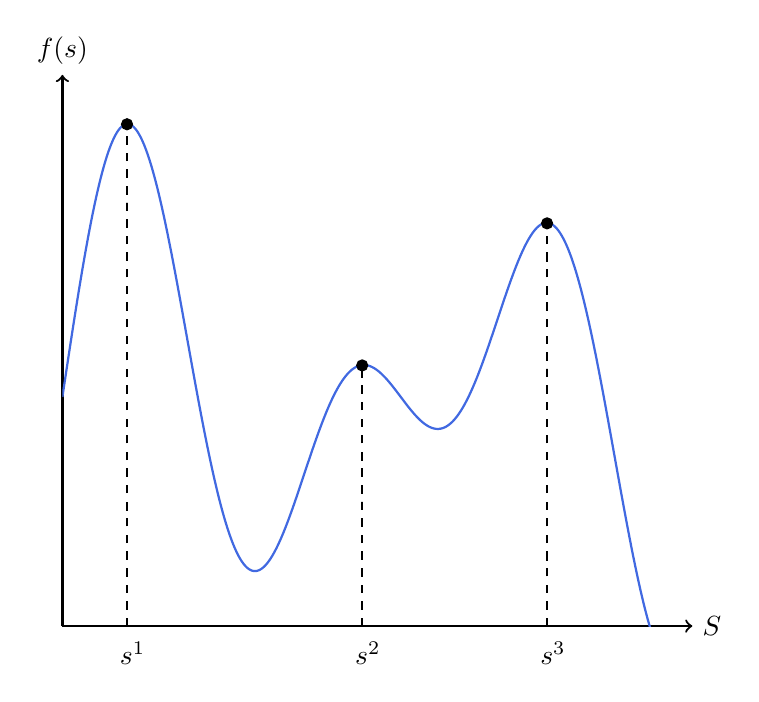
\begin{tikzpicture}
	% Axis Lines
	\draw[->, thick] (0,0) -- (8,0) node[right] {$S$};
	\draw[->, thick] (0,0) -- (0,7) node[above] {$f(s)$};

	\begin{axis}[axis lines = none,scale only axis=true,xmin=0,
			xmax=18.5,ymin=0,ymax=10]

		% Main Plot
		\addplot[domain=0:17,samples=1000,smooth,color=RoyalBlue,
			thick] {2.5*sin(deg(x)) + 2.5*sin(deg((2/3)*x)) + 4};

		% Vertical Line (s1)
		\addplot[domain=0:17,thick,samples=1000,dashed,
			smooth] coordinates {(1.8,0) (1.8,8.76)};
		\addplot[domain=0:17,mark=*] coordinates {(1.8,8.76)};
		% \draw (1.8,8.76) circle[radius=1.5pt];
		% \fill (1.8,8.76) circle[radius=1.5pt];

		% Vertical Line (s2)
		\addplot[domain=0:17,thick,samples=1000,dashed,
			smooth] coordinates {(8.35,0) (8.35,4.55)};
		% \draw (8.35,4.55) circle[radius=1.5pt];
		% \fill (8.35,4.55) circle[radius=1.5pt];
		\addplot[domain=0:17,mark=*] coordinates {(8.35,4.55)};

		% Vertical Line (s3)
		\addplot[domain=0:17,thick,samples=1000,dashed,
			smooth] coordinates {(13.5,0) (13.5,7.03)};
		% \draw (13.5,7.03) circle[radius=1.5pt];
		% \fill (13.5,7.03) circle[radius=1.5pt];
		\addplot[domain=0:17,mark=*] coordinates {(13.5,7.03)};
	\end{axis}

	% Labels
	\node (s1) at (0.89,-0.35) {$s^1$};
	\node (s1) at (3.88,-0.35) {$s^2$};
	\node (s1) at (6.23,-0.35) {$s^3$};

\end{tikzpicture}


  \caption{Global and Local Optima}
  \label{fig:optima}
\end{figure}

In practice, the decision to use either a global or local optimization strategy
is often influenced by factors such as the available time budget and the
preferences of the decision maker. While~\acrshort{global-optimization} aims to
find the optimal solution to a problem, the search process may be time-consuming
or, in some cases, computationally infeasible due to the size of the search
space.  On the other hand,~\acrshort{local-optimization}, while lacking the
optimality guarantees of, is able to quickly generate~\textquote{good} solutions that may be
acceptable to the decision maker. Nonetheless, the quality of the solutions may
be poor due to the ruggedness of the objective function fitness landscape (many
local optima). Ultimately, the performance of both methods is closely tied to
problem-specific knowledge.

In the Google Hash Code competition, due to the time imposed by the competition
setting, it is often not in the interest of the contestants to use global
optimization methods, as they are unlikely to finish on more complex problem
instances. Instead, a balance between global and local optimization
(\textit{exploration} and \textit{exploitation}) is typically employed. To
elaborate, the strategy typically involves~\textit{exploring} the search space
via~\acrshort{global-optimization} methods to find~\textquote{good} starting
solutions, which~\acrshort{local-optimization} methods can
further~\textit{exploit}.

\subsection{Black-Box and Glass-Box Optimization}
\label{subsec:bbo-and-gbo}

In the field of optimization, two settings are commonly recognized:
\acrfull{black-box-optimization} and \acrfull{glass-box-optimization}.

In~\acrshort{black-box-optimization} optimization settings there is no
information about the landscape of the function being optimized, constraints
defining the set of feasible solutions~\cite{alarie2021two}, or the objective
function is too complex to be approached from an analytical perspective. As
such, algorithms to solve these problems do so only by interacting with the
problem through the evaluation of potential candidate
solutions~\cite{doerr2020complexity,gutjahr2010stochastic}.~Meta-Heuristics, as
will be later detailed are examples of methods that follow this approach for
finding/improving solutions.~By contrast, in~\acrshort{glass-box-optimization}
optimization, also known as~\textit{white box} optimization, there is a good
understanding of the problem instance being optimized and the objective function
properties~\cite{doerr2020complexity}. Hence, the algorithms used may take
advantage of more analytical properties of the problem since they are
transparent to the solver.

% For the purpose of clarification, with regard to the previously mentioned
% ~\acrshort{knapsack-problem}, a~\acrshort{black-box-optimization} strategy would
% entail the utilization of a search heuristic such as simulated
% annealing~\cite{luke2013essentialsa} to obtain solutions. This is because the
% algorithm only necessitates knowledge of how to evaluate the quality of
% solutions through the objective function and not any specific information about
% the function being optimized. Alternatively, if the problem were to be
% formulated as an~\acrfull{ilp}~\cite{nocedal2006numerical,papadimitriou1998combinatorial}
% problem, it would become amenable to a~\acrshort{glass-box-optimization}
% approach, as the objective function would be accessible, and additional
% information about the problem could be inferred from it and provided to the
% algorithm.

In the context of the Hash Code competition, contestants typically engage the
problems from a~\acrshort{black-box-optimization} perspective, as the underlying
objective function of the is too complex to formalize. Additionally, the process
of formalization can be time-consuming and, as a result, the usage of
~\acrshort{glass-box-optimization} methods post-formalization would not be
justified, as they could turn out to be computationally slower. However, it is
in many cases, possible to use~\acrshort{glass-box-optimization}
methods,~\eg{},~\acrfull{ilp} to tackle sub-problems that are simpler to
formalize.